\subsection{Optimizations}

\begin{frame}
	% LIMIT NUMBER OF PARENTS
	\begin{itemize}
		\item Limit the maximum number of parents for each variable
	\end{itemize}
	\begin{block}{Theorem 1}
		In an optimal Bayesian network based on the BIC scoring function, each
variable has at most $d = \lfloor log( \frac{ 2N }{ log N } ) \rfloor$ parents, where $N$ is the number of instances.
	\end{block}
	\pause
	% PRUNE NOT OPTIMUM PARENT SETS
	\begin{itemize}
		\item Prune non-optimal candidate parent sets
	\end{itemize}
	\begin{block}{Theorem 2}
		Let $U$ and $S$ be two candidate parent sets for $X$ such that $U \subset S$, and ${sc}( X , U )$ is \alert{better} than ${sc}( X , S )$. Then $S$ is not the optimal parent set of $X$ for any candidate set.
	\end{block}
\end{frame}

\begin{frame}
	\begin{table}
	\centering
	\begin{tabular}{ | l | c | c | }
		\hline
		Dataset & n (\#attributes) & N (\#instances) \\ \hline
		Census & 15 & 30168 \\ \hline
		Voting & 17 & 232 \\ \hline
		Letter & 17 & 20000 \\ \hline
		Hepatitis & 17 & 80 \\ \hline
		Image & 20 & 2310 \\ \hline
		Heart & 23 & 80 \\ \hline
		Mushroom & 23 & 8124 \\ \hline
		Parkinsons & 23 & 195 \\ \hline
		Autos & 25 & 159 \\ \hline
		Flag & 28 & 194 \\ \hline
	\end{tabular}
	\caption{Data sets characteristics}
	\label{tab:datasets}
\end{table}
\end{frame}

\begin{frame}
	\begin{figure}
		\centering
		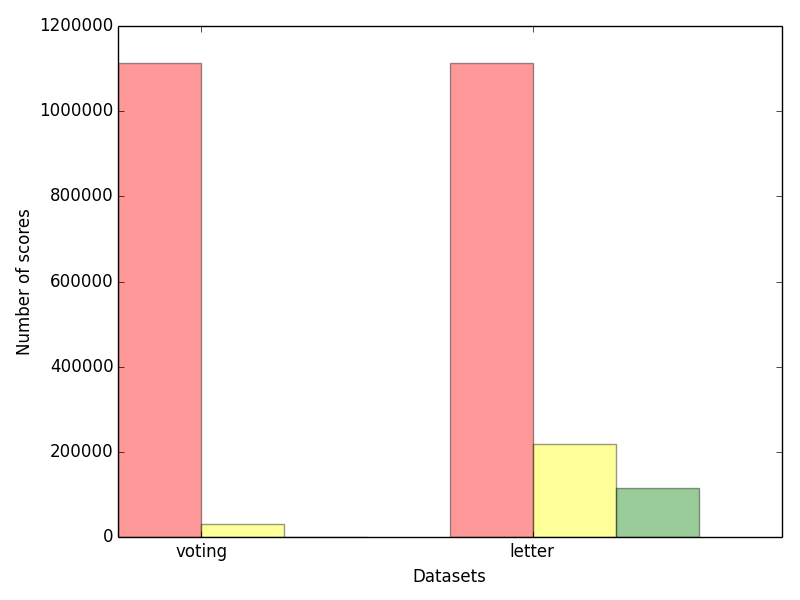
\includegraphics[height=7cm]{images/num_scores}
	\end{figure}
\end{frame}

\begin{frame}
	\begin{table}
	\centering
	\resizebox{\columnwidth}{!}{%
	\begin{tabular}{ | l | c | c | c | c | }
		\hline
		Dataset & d & Total Scores & Limited Scores & Pruned Scores \\ \hline
		Census & 8 & 245K & 45K (18.33\%) & 3.5K (1.44\%) \\ \hline
		Voting & 4 & 1.1M & 31K (2.78\%) & 939 (0.08\%) \\ \hline
		Letter & 8 & 1.1M & 218K (19.64\%) & 115K (10.38\%) \\ \hline
		Hepatitis & 3 & 1.1M & 9.5K (0.85\%) & 174 (0.02\%) \\ \hline
		Image & 6 & 10M & 542K (5.18\%) & 6.2K (0.06\%) \\ \hline
		Heart & 3 & 96M & 35K (0.04\%) & 327 (0.00034\%) \\ \hline
		Mushroom & 7 & 96M & 3.9M (4.07\%) & 13K (0.014\%) \\ \hline
		Parkinsons & 4 & 96M & 168K (0.17\%) & 2.4K (0.003\%) \\ \hline
		Autos & 4 & 419M & 265K (0.06\%) & 3K (0.0007\%) \\ \hline
		Flag & 4 & 3.7B & 491K (0.01\%) & 776 (0.00002\%) \\ \hline
	\end{tabular}%
	}
	\caption{Number of scores}
	\label{tab:num_scores}
\end{table}
\end{frame}